\documentclass[12pt, a4paper, oneside, UTF8]{ctexart}
\usepackage{amsmath, amsthm, amssymb, bm, color, framed, graphicx, hyperref, mathrsfs}
\usepackage{geometry}
\geometry{left = 2.5 cm, right = 2.5 cm, top = 2.5 cm, bottom = 2.5 cm}

\title{\textbf{作业7}\\{\small (数值算法与案例分析)}}
\author{李维杰}
\date{ 2024年 10 月 30 日 }
\linespread{1.5}
\definecolor{shadecolor}{RGB}{241, 241, 255}
\newcounter{problemname}
\newenvironment{problem}{\begin{shaded}\stepcounter{problemname}\par\noindent\textbf{题目\arabic{problemname}. }}{\end{shaded}\par}
\newenvironment{solution}{\par\noindent\textbf{解答. }}{\par}
\newenvironment{note}{\par\noindent\textbf{注记. }}{\par}

\begin{document}

\maketitle

\begin{problem}
    设$(\hat{\lambda},\hat{x})$是$A \in \mathbb{C}^{n \times n}$的一个近似特征对,并设残差$r = A\hat{x} -\hat{x}\hat{\lambda}$.
    假设${\left\lVert{x}\right\rVert}_{2}=1$.证明存在一个满足${\left\lVert{E}\right\rVert}_{2} \leq {\left\lVert{r}\right\rVert}_{2}$的矩阵$E \in \mathbb{C}^{n \times n}$,使得
    $$(A+E)\hat{x}=\hat{x}\hat{\lambda}.$$
\end{problem}

\begin{solution}
    构造$E=-r{\hat{x}}^*$,则满足
    \begin{align*}
        {\left\lVert{E}\right\rVert}_{2} &= {\left\lVert{r{\hat{x}}^*}\right\rVert}_{2} \\
        &\leq {\left\lVert{r}\right\rVert}_{2}{\left\lVert{\hat{x}}\right\rVert}_{2} \\
        &= {\left\lVert{r}\right\rVert}_{2}
    \end{align*}
    且有
    \begin{align*}
        (A+E)\hat{x} &= (A - r{\hat{x}}^*)\hat{x} \\
        &= A\hat{x} -r{\left\lVert{x}\right\rVert}_{2}^{2} \\
        &= A\hat{x} - r\\
        &= \hat{x}\hat{\lambda}.
    \end{align*}
\end{solution}
\newpage
\begin{problem}
    设$A_0 \in \mathbb{C}^{n \times n}$,以及${\mu}_0,{\mu}_1,...,{\mu}_m \in \mathbb{C}$. 通过下列递归定义$A_1,A_2,...,A_{m+1}$
    \begin{align*}
        \left\{
            \begin{array}{ll}
                A_k-{{\mu}_k}I = {Q_k}{R_k} \\
                A_{k+1} = {R_k}{Q_k}+{{\mu}_k}I
            \end{array}
        \right.,
    \end{align*}
    其中$Q_k$是正交阵.证明
    \begin{align}
        \prod_{k=0}^{m}{(A_0-{{\mu}_k}I)} = (\prod_{k=0}^{m}{Q_k})(\prod_{k=0}^{m}{R_{m-k}})
    \end{align}
\end{problem}

\begin{solution}
    对$m$采用数学归纳法,当$m=0$时,有$$A_0-{{\mu}_0}I={Q_0}{R_0},$$显然符合(1)式.\\
    假设当$m=m_0$时,(1)式成立,即可推得
    \begin{align*}
        \prod_{k=1}^{m_0+1}{(A_1-{{\mu}_k}I)} = (\prod_{k=1}^{m_0+1}{Q_k})(\prod_{k=1}^{m_0+1}{R_{m_0+2-k}}).
    \end{align*}
    下面考虑当$m=m_0+1$的情况下(1)式是否成立.由于
    \begin{align*}
        Q_{0}(A_{1}-{{\mu}_k}I)Q_{0}^{*} &= Q_{0}({R_0}{Q_0}+({\mu}_0-{\mu}_k)I)Q_{0}^{*} \\
        &= {Q_0}{R_0} + ({\mu}_0-{\mu}_k)I \\
        &= A_{0} - {{\mu}_k}I.
    \end{align*}
    于是有
    \begin{align*}
        \prod_{k=0}^{m_0+1}{(A_0-{{\mu}_k}I)} &= (\prod_{k=1}^{m_0+1}{(A_0-{{\mu}_k}I)})(A_0-{{\mu}_0}I) \\
        &= Q_{0}(\prod_{k=1}^{m_0+1}{(A_1-{{\mu}_k}I)})Q_{0}^{*}(A_0-{{\mu}_0}I) \\
        &= (\prod_{k=1}^{m_0+1}{Q_k})(\prod_{k=1}^{m_0+1}{R_{m_0+2-k}})Q_{0}^{*}(A_0-{{\mu}_0}I)Q_{0} \\
        &= (\prod_{k=1}^{m_0+1}{Q_k})(\prod_{k=1}^{m_0+1}{R_{m_0+2-k}})Q_{0}^{*}Q_{0}R_{0} \\
        &= (\prod_{k=0}^{m_0+1}{Q_k})(\prod_{k=0}^{m_0+1}{R_{m_0+1-k}}).
    \end{align*}
    于是原命题得证.
\end{solution}

\begin{problem}
    随机生成一个$1000 \times 1000$的正元素矩阵$A$. 使用power method计算$\rho(A)$. 可视化收敛过程.
\end{problem}

\begin{solution}
    (代码见Problem3.m)
    \begin{figure}[htbp] % 创建一个图形环境
        \centering % 图片居中
        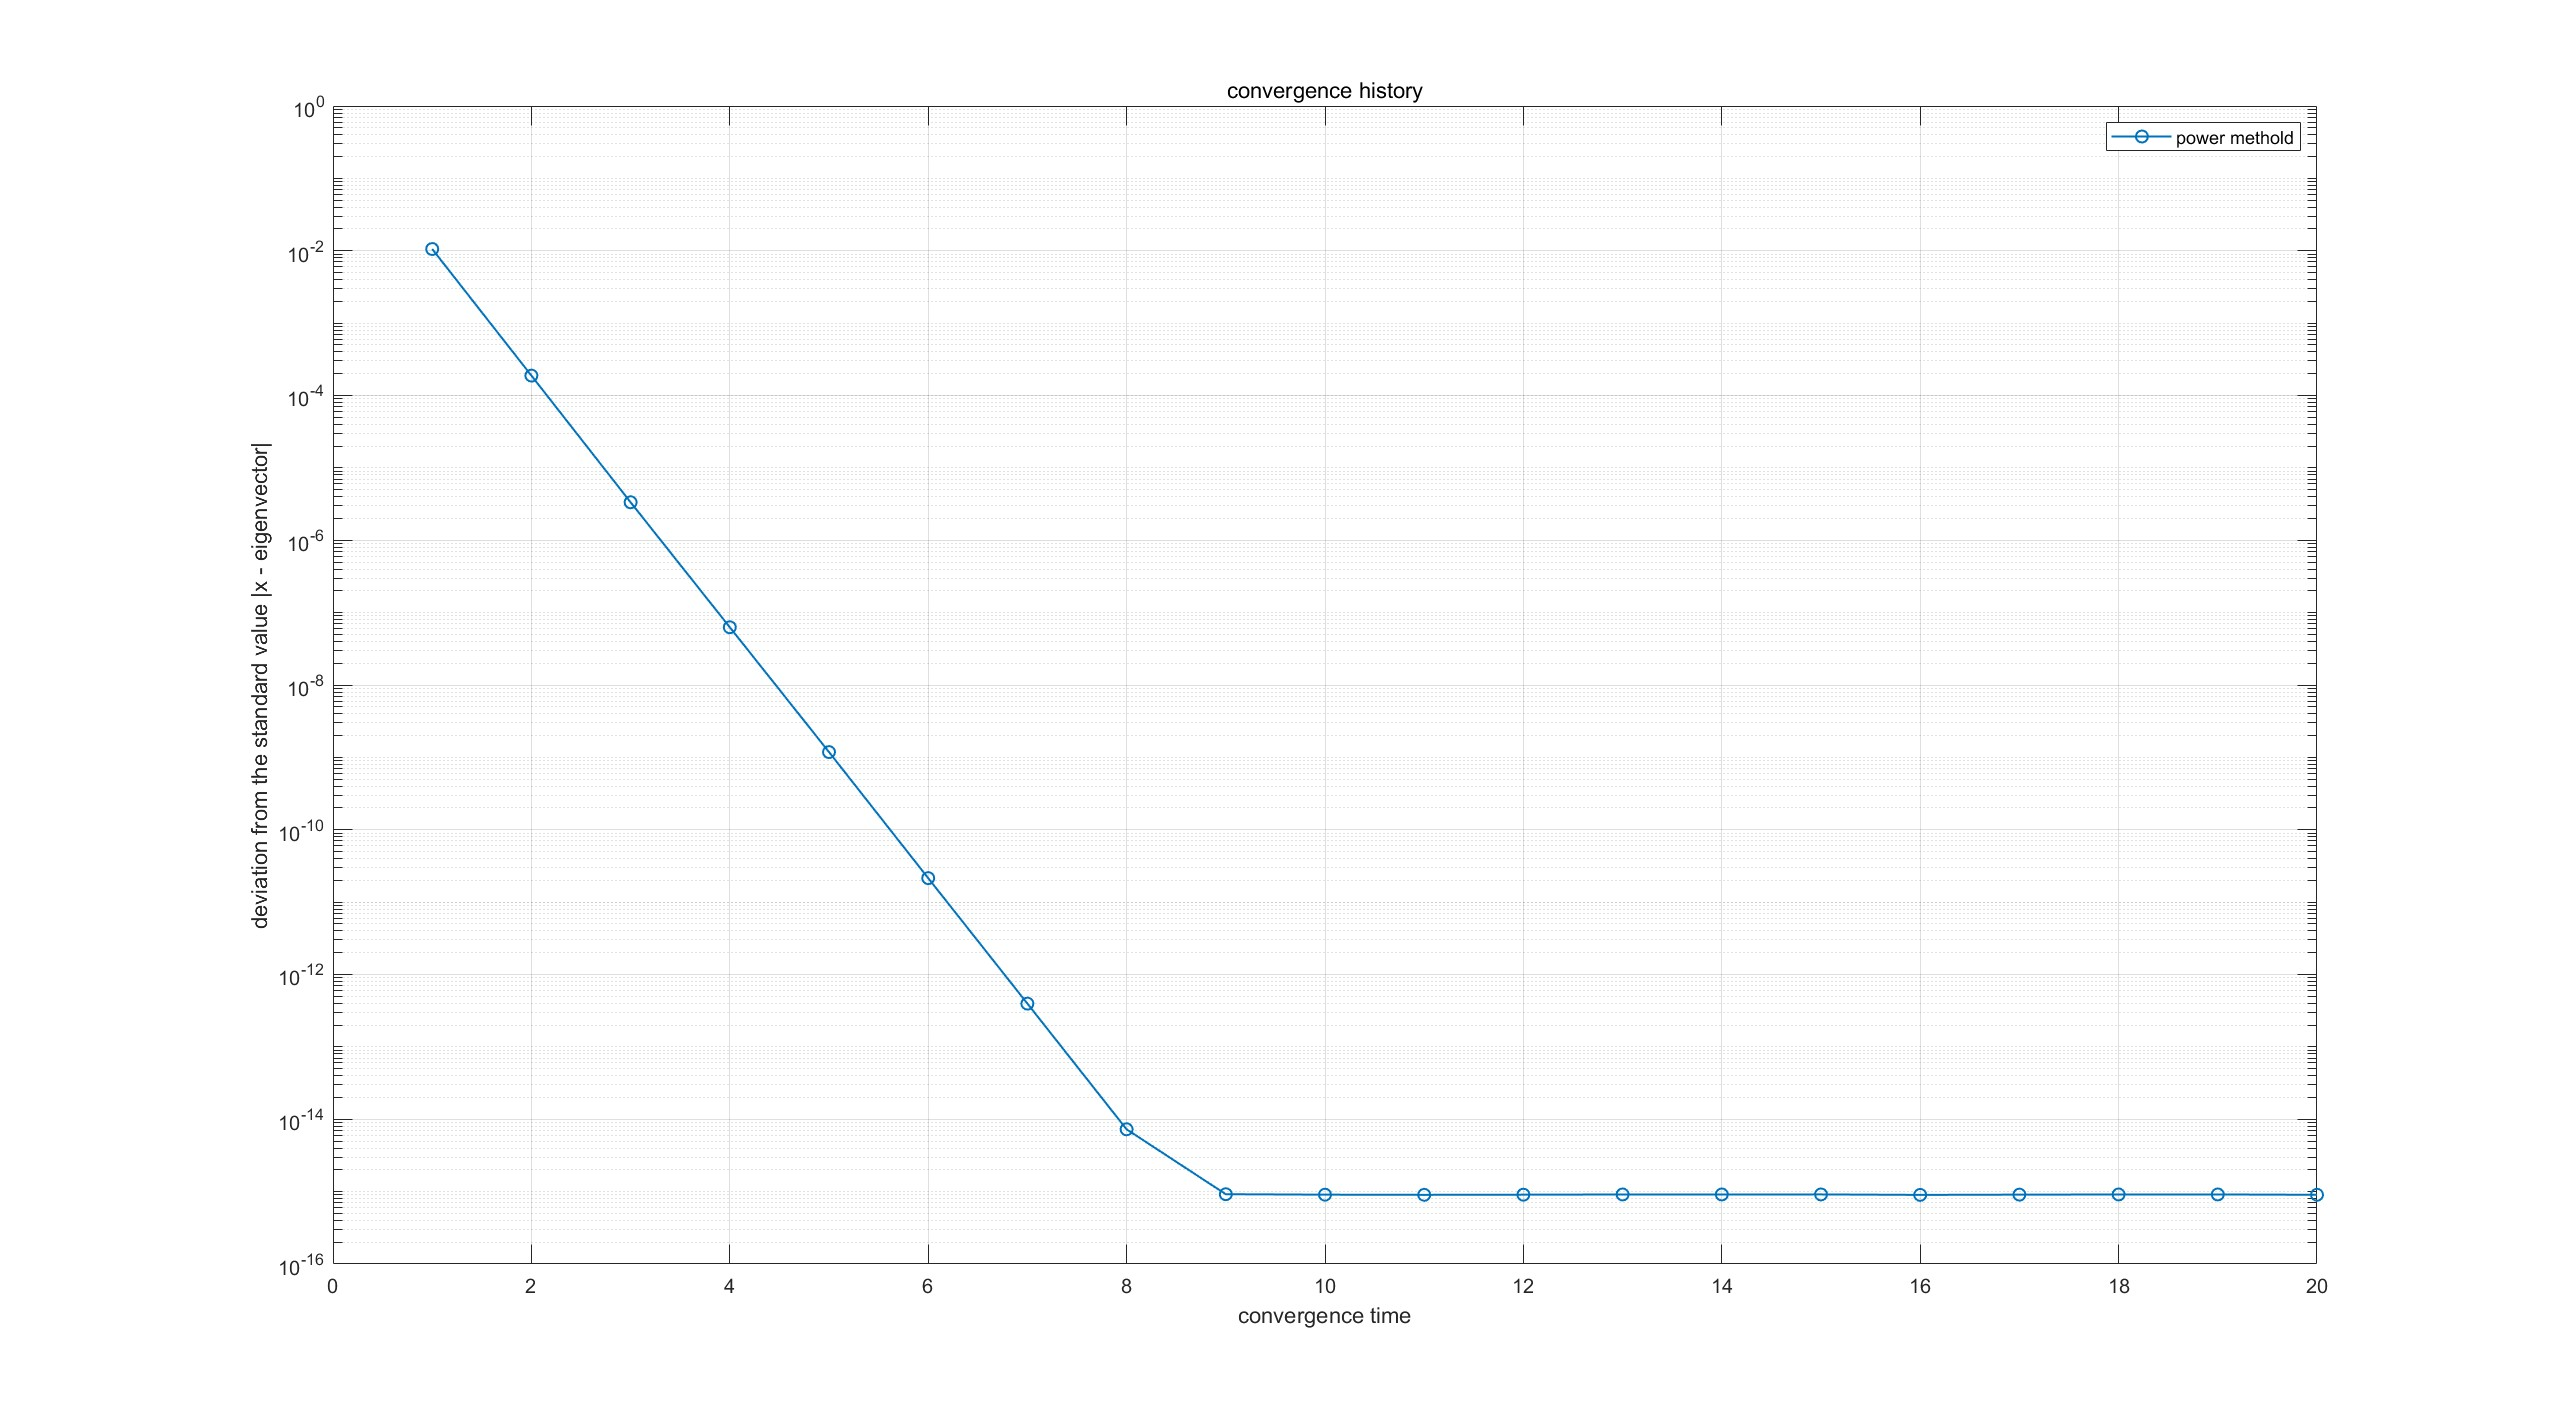
\includegraphics[scale=0.16]{Problem3.jpg} % 插入图片,设置宽度为页面宽度的70%
        \caption{收敛过程(以${\left\lVert{\hat{x}-x}\right\rVert}_{2}$衡量收敛程度)} % 图片的说明文字
    \end{figure}
\end{solution}

\begin{problem}
    设$A$是一个$200 \times 200$的Hilbert矩阵(满足$a_{ij}=(i+j-1)^{-1}$).分别使用inverse iteration和Rayleigh quotient iteration计算$A$最接近$1$的特征值.
    可视化收敛过程并指出算法的耗时(最好附带详细的分析)
\end{problem}

\begin{solution}
    (代码见Problem4.m)\par
    对于inverse iteration, 算法在预处理中即先求出了$(A-I)$的$LU$分解,这一处理的时间复杂度为$O(n^3)$.
    在每一步迭代中,均需要进行两步解三角线性方程组,单次迭代的时间复杂度为$O(n^2)$.设迭代次数为$m$,则此算法的总时间复杂度为$O(n^3)+O(mn^2).$\par
    对于Rayleigh quotient iteration, 算法在每一步迭代中均需要解一个线性方程组,这一操作的时间复杂度为$O(n^3)$,同时每一步操作均需要计算一次Rayleigh商,这一操作的时间复杂度为$O(n)$.
    设迭代次数为$m$,则此算法的总时间复杂度为$O(mn^3)$.
    \begin{figure}[htbp] % 创建一个图形环境
        \centering % 图片居中
        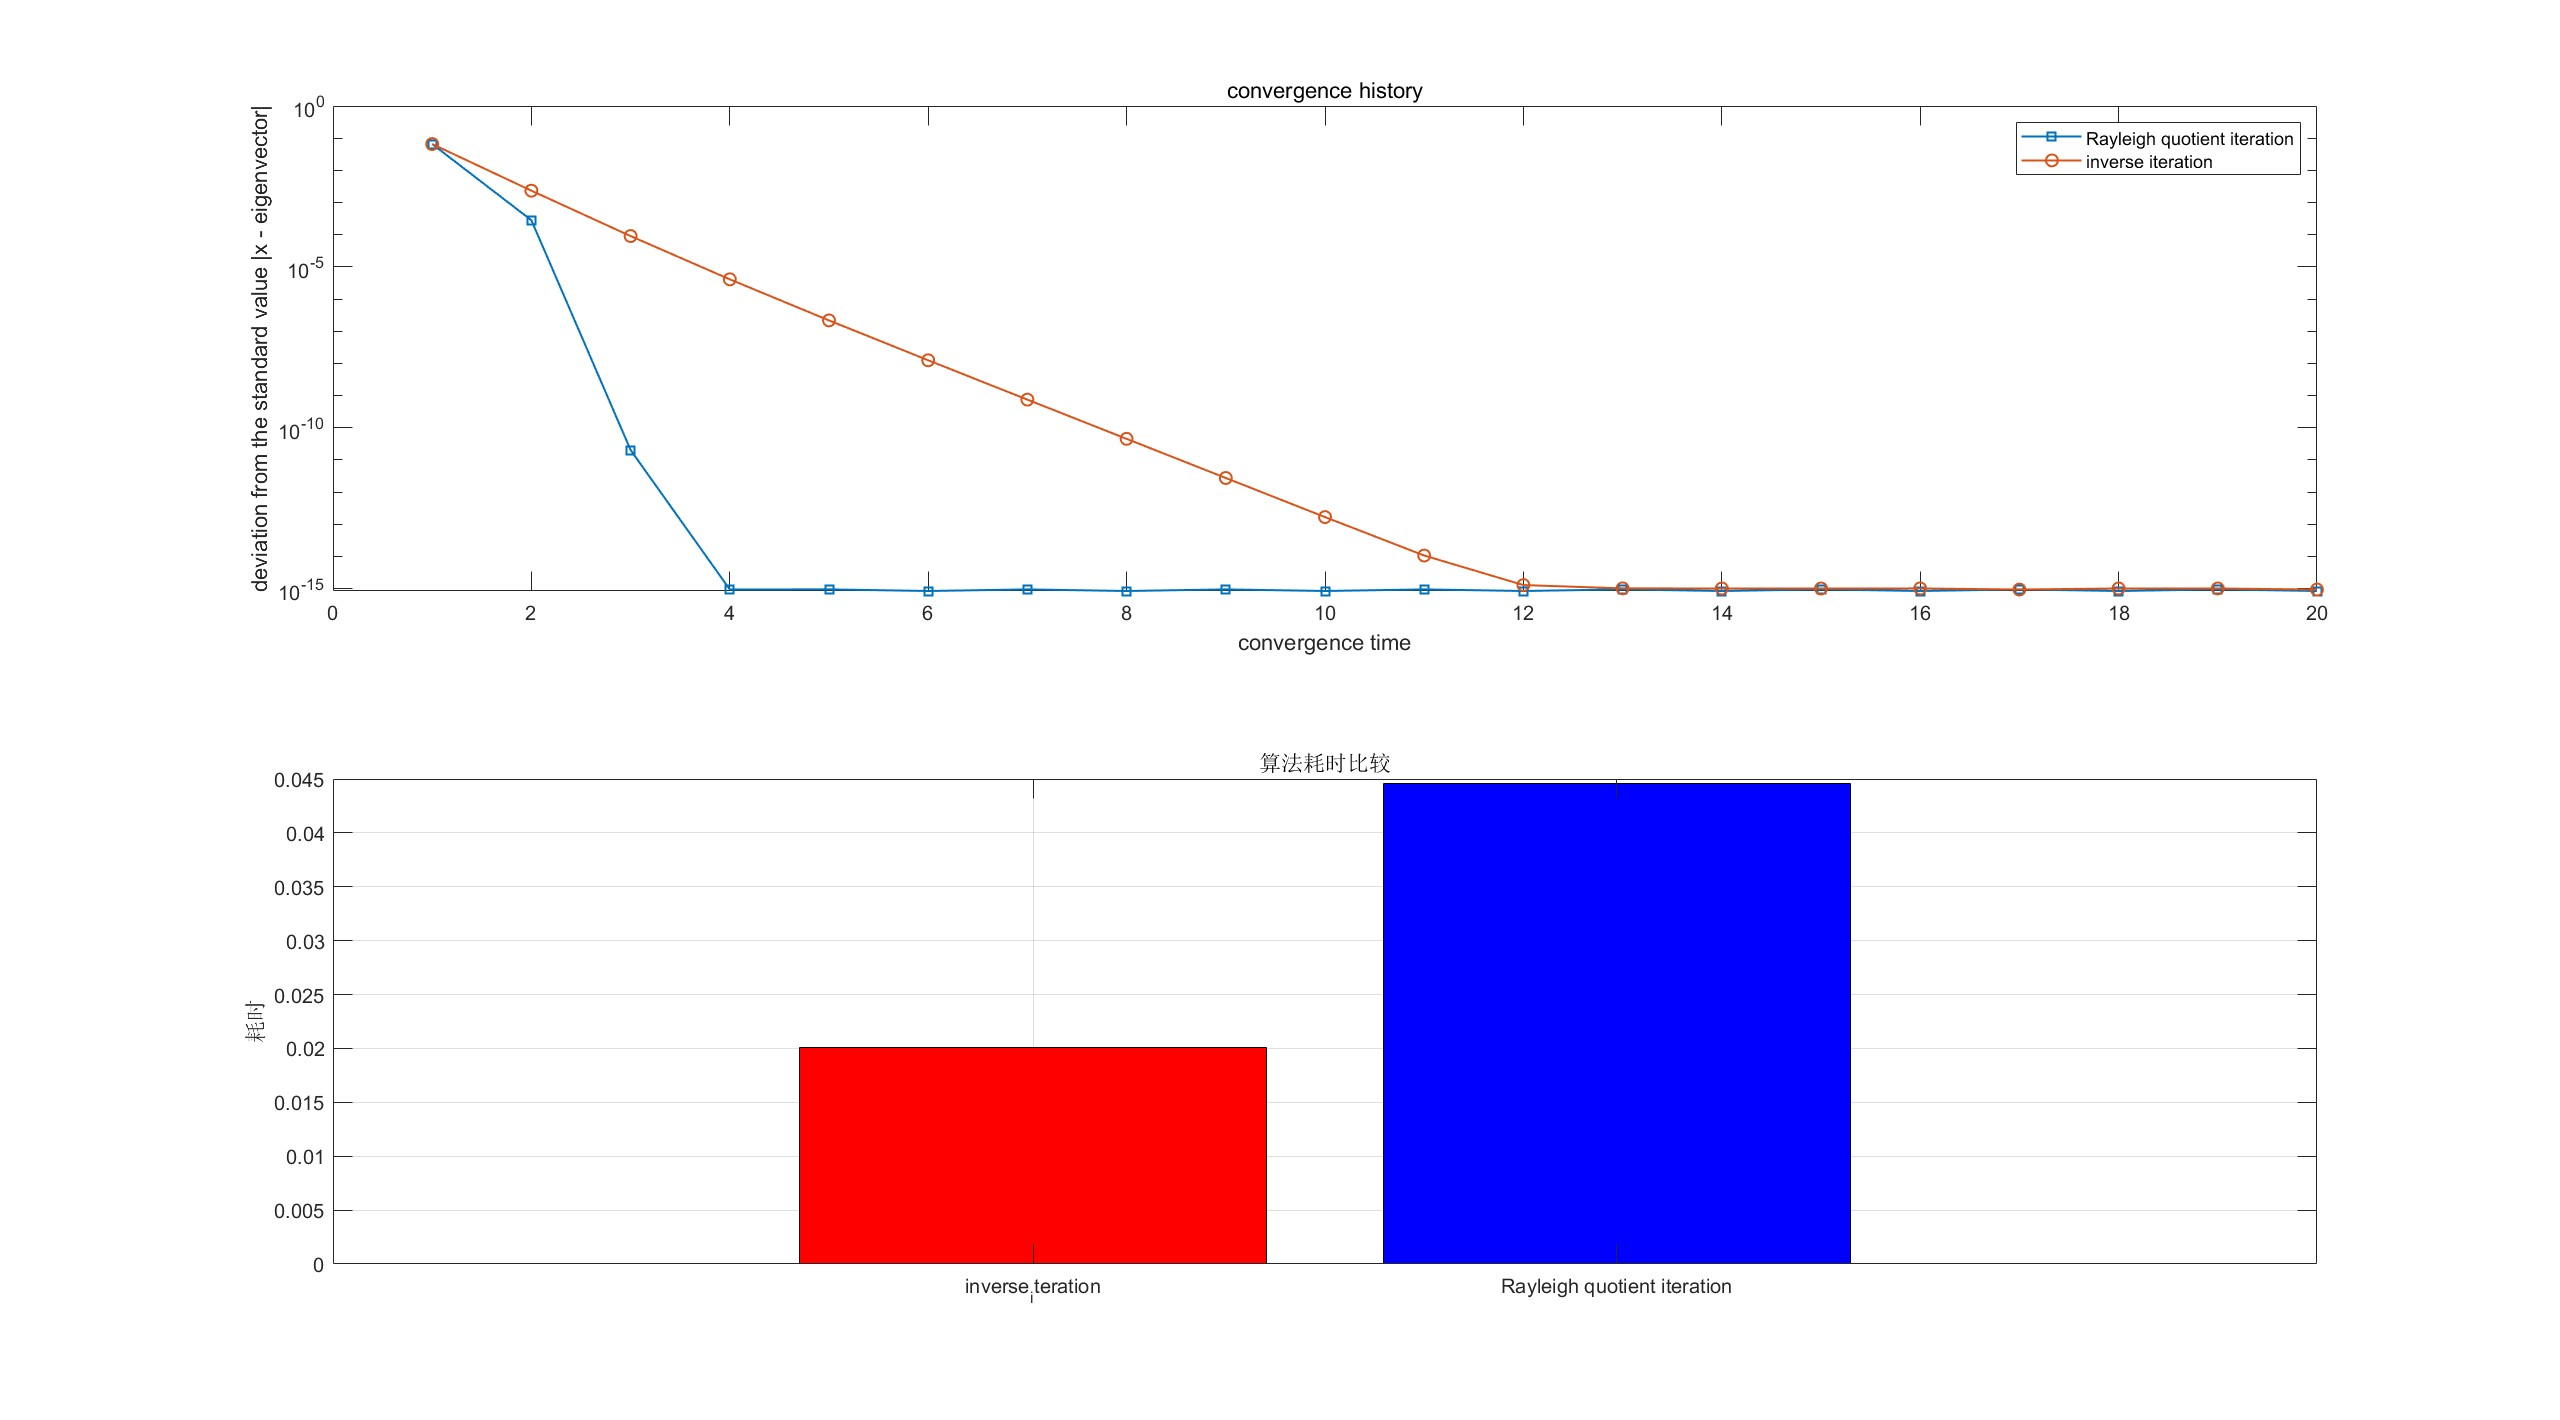
\includegraphics[scale=0.16]{Problem4.jpg} % 插入图片,设置宽度为页面宽度的70%
        \caption{两种算法的收敛速度和消耗时间} % 图片的说明文字
    \end{figure}
\end{solution}

\begin{problem}
    写一个程序来计算一个拥有不同对角元素的上三角阵的所有特征值.并把程序得到的结果与MATLAB自带的$\textbf{eig}$函数得到的结果做比较.
\end{problem}

\begin{solution}
    (代码见Problem5.m)
    \begin{figure}[htbp] % 创建一个图形环境
        \centering % 图片居中
        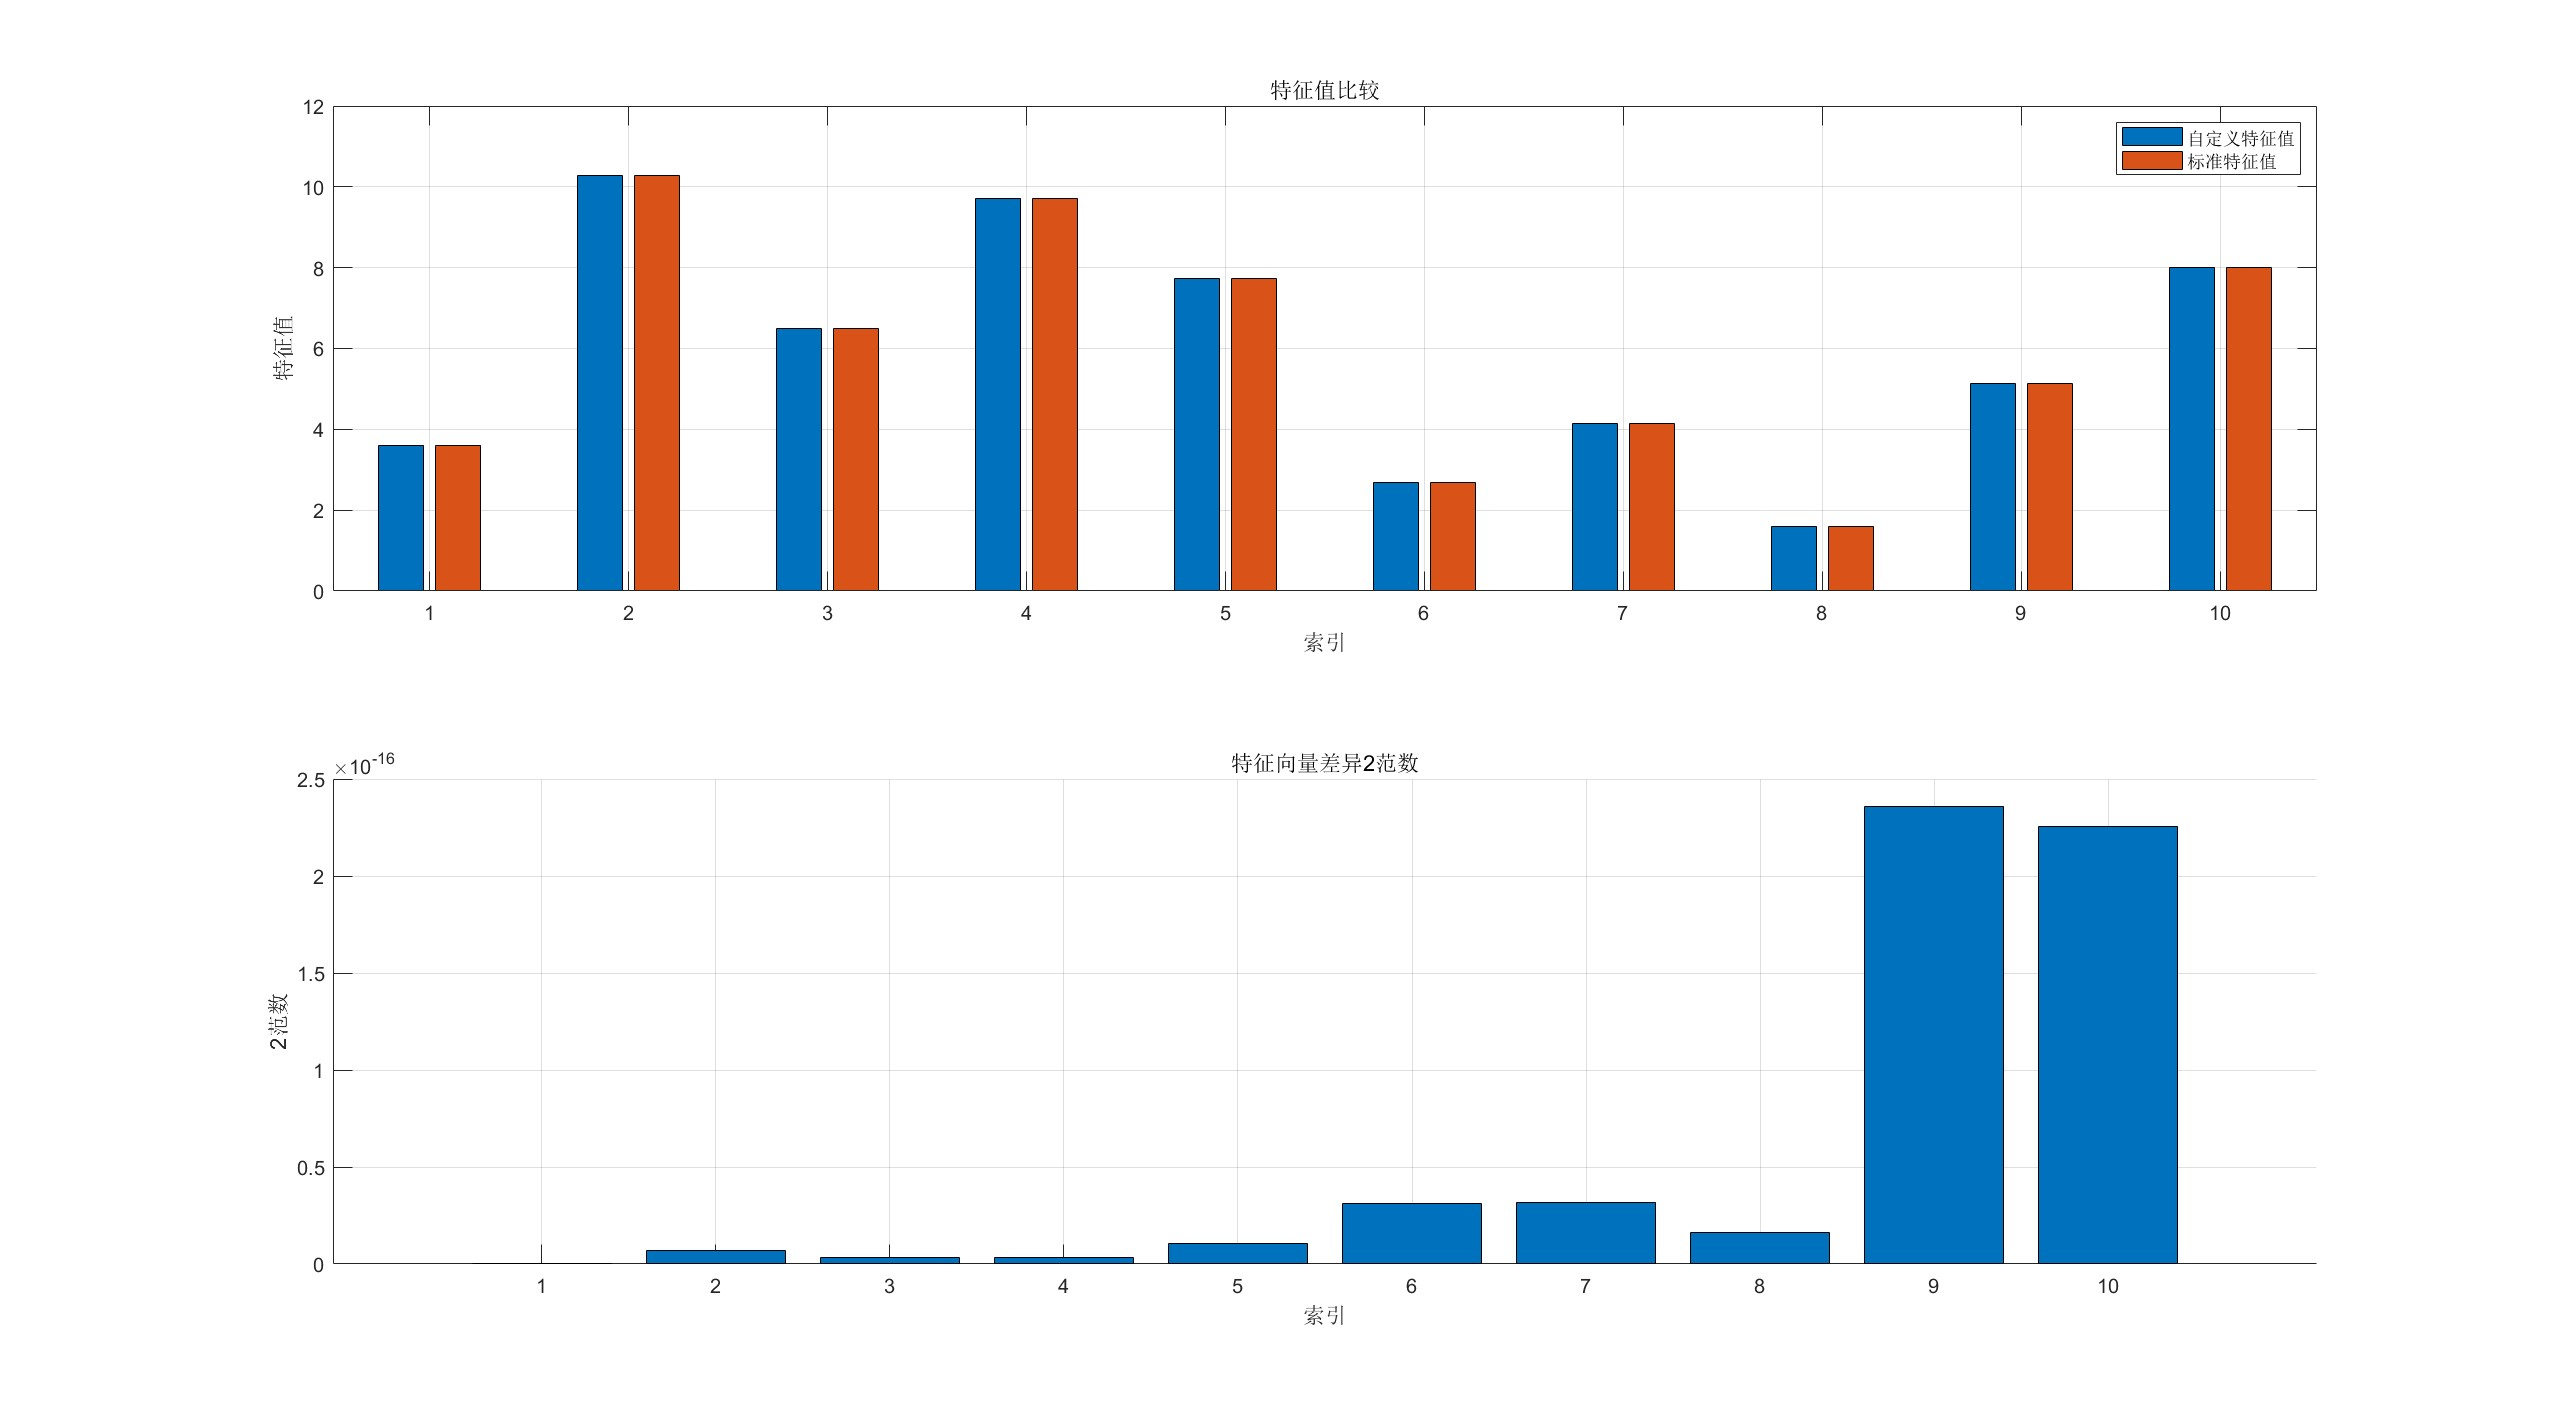
\includegraphics[scale=0.16]{Problem5.jpg} % 插入图片,设置宽度为页面宽度的70%
        \caption{程序结果与标准函数库结果的差异情况} % 图片的说明文字
    \end{figure}
\end{solution}
\end{document}